\documentclass{beamer}
\usepackage[utf8]{inputenc}

\usetheme{Madrid}
\usecolortheme{default}
\usepackage{amsmath,amssymb,amsfonts,amsthm}
\usepackage{txfonts}
\usepackage{tikz}
\usepackage{graphicx}
\usepackage{mathtools} 
\setbeamertemplate{page number in head/foot}[totalframenumber]

\newcommand{\myvec}[1]{\begin{pmatrix}#1\end{pmatrix}}
\let\vec\mathbf

\title{9.4.17}
\author{EE25BTECH11005 - Aditya Mishra}
\date{\today}

\begin{document}

\frame{\titlepage}

\begin{frame}{Question}
Find the roots of the quadratic equation graphically
\[
2x^2 + x - 4 = 0
\]
\end{frame}

\begin{frame}{Matrix Representation}
Write the quadratic as a conic in matrix form:
\[
\vec{x}^{\top} \vec{V} \vec{x} + 2 \vec{u}^{\top} \vec{x} + f = 0
\]
where
\[
\vec{V} = \myvec{2 & 0 \\ 0 & 0}, \quad
\vec{u} = \myvec{\frac{1}{2} \\ 0}, \quad
f = -4
\]
\end{frame}

\begin{frame}{Roots via Line Intersection}
The roots correspond to intersection points of the conic with the x-axis:
\[
\vec{x} = \vec{h} + k \vec{m}
\]
where
\[
\vec{h} = \myvec{0 \\ 0}, \quad \vec{m} = \myvec{1 \\ 0}.
\]
\end{frame}

\begin{frame}{Solving for \(k\)}
The value of $k$ can be found by solving the line and conic equation:
\begin{align}
(\vec{h} + k \vec{m})^{\top} \vec{V} (\vec{h} + k \vec{m}) + 2\vec{u}^{\top} (\vec{h} + k \vec{m}) + f &= 0 \\
\implies k^{2} \vec{m}^{\top}\vec{V}\vec{m} + 2k \vec{m}^{\top} (\vec{V}\vec{h} + \vec{u}) + g(\vec{h}) &= 0
\end{align}
\end{frame}

\begin{frame}{Solution for \(k\)}
Solving the quadratic formula:
\begin{align}
k = \frac{1}{\vec{m}^{\top}\vec{V}\vec{m}}
\Bigg[
    -\vec{m}^{\top} (\vec{V}\vec{h} + \vec{u})
    \pm
    \sqrt{ (\vec{m}^{\top}(\vec{V}\vec{h} + \vec{u}))^2 - g(\vec{h}) (\vec{m}^{\top}\vec{V}\vec{m}) }
\Bigg]
\end{align}

Substitute values for our quadratic:
\[
\vec{V} = \myvec{2 & 0 \\ 0 & 0}, \quad
\vec{u} = \myvec{\frac{1}{2} \\ 0}, \quad
f = -4, \quad
\vec{h} = \myvec{0 \\ 0}, \quad
\vec{m} = \myvec{1 \\ 0}
\]

\[
\vec{m}^{\top} \vec{V} \vec{m} = 2, \quad
\vec{m}^{\top}(\vec{V}\vec{h} + \vec{u}) = \frac{1}{2}, \quad
g(\vec{h}) = -4
\]

\[
\therefore k = \frac{1}{2} \Big[-\frac{1}{2} \pm \sqrt{\frac{1}{4}+8} \Big] = \frac{1}{2} \Big[-\frac{1}{2} \pm \sqrt{\frac{33}{4}} \Big]
\]

\[
k_1 = \frac{-1 + \sqrt{33}}{4} \approx 1.186, \quad
k_2 = \frac{-1 - \sqrt{33}}{4} \approx -1.686
\]
\end{frame}

\begin{frame}{Roots of the Quadratic}
The intersection points:
\[
\vec{x}_1 = \vec{h} + k_1 \vec{m} = \myvec{1.186 \\ 0}, \quad
\vec{x}_2 = \vec{h} + k_2 \vec{m} = \myvec{-1.686 \\ 0}
\]

\[
\Rightarrow \text{The roots of } 2x^2 + x - 4 = 0 \text{ are } x \approx 1.186 \text{ and } x \approx -1.686
\]
\end{frame}
\begin{frame}{Graphical Representaion}
\begin{figure}[h!]
    \centering
    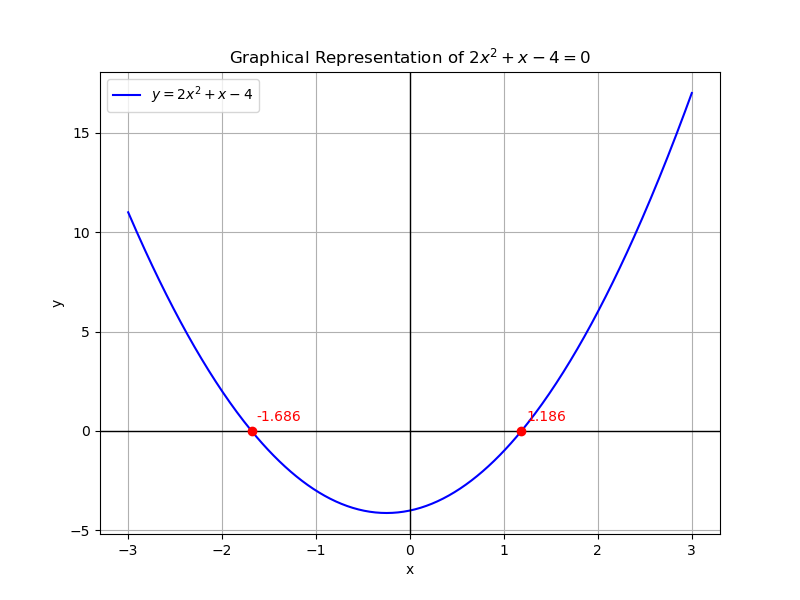
\includegraphics[height=0.5\textheight, keepaspectratio]{Figs/Figure_1.png}
    \caption{Graph of $2x^2 + x - 4 = 0$ showing its roots.}
    \label{figure_1}
\end{figure}
\end{frame}


\begin{frame}[fragile]{Codes}
For Codes, please refer to:
\url{https://github.com/AdityaMishra11005/ee1030-2025/tree/main/ee25btech11005/matgeo/9.4.17/Codes}
\end{frame}

\end{document}

